\section{Vectores}
  \subsection{Sistemas coordenados}
    \PN En el sistema de coordenadas polares $(r, \theta)$, $r$ es la distancia desde el origen hasta el punto que tiene
    coordenadas cartesianas (x, y) y $\theta$ es el ángulo entre un eje fijo y una recta dibujada desde el origen hasta
    el punto. El eje fijo es el eje x positivo y $\theta$ se mide contra el sentido de las agujas del reloj.
    \begin{eqnarray*}
      x = r \ cos(\theta) \\
      y = r \ sen(\theta) \\
      r = \sqrt{x^{2} + y^{2}}
    \end{eqnarray*}

    \begin{figure}[H]
      \centering
      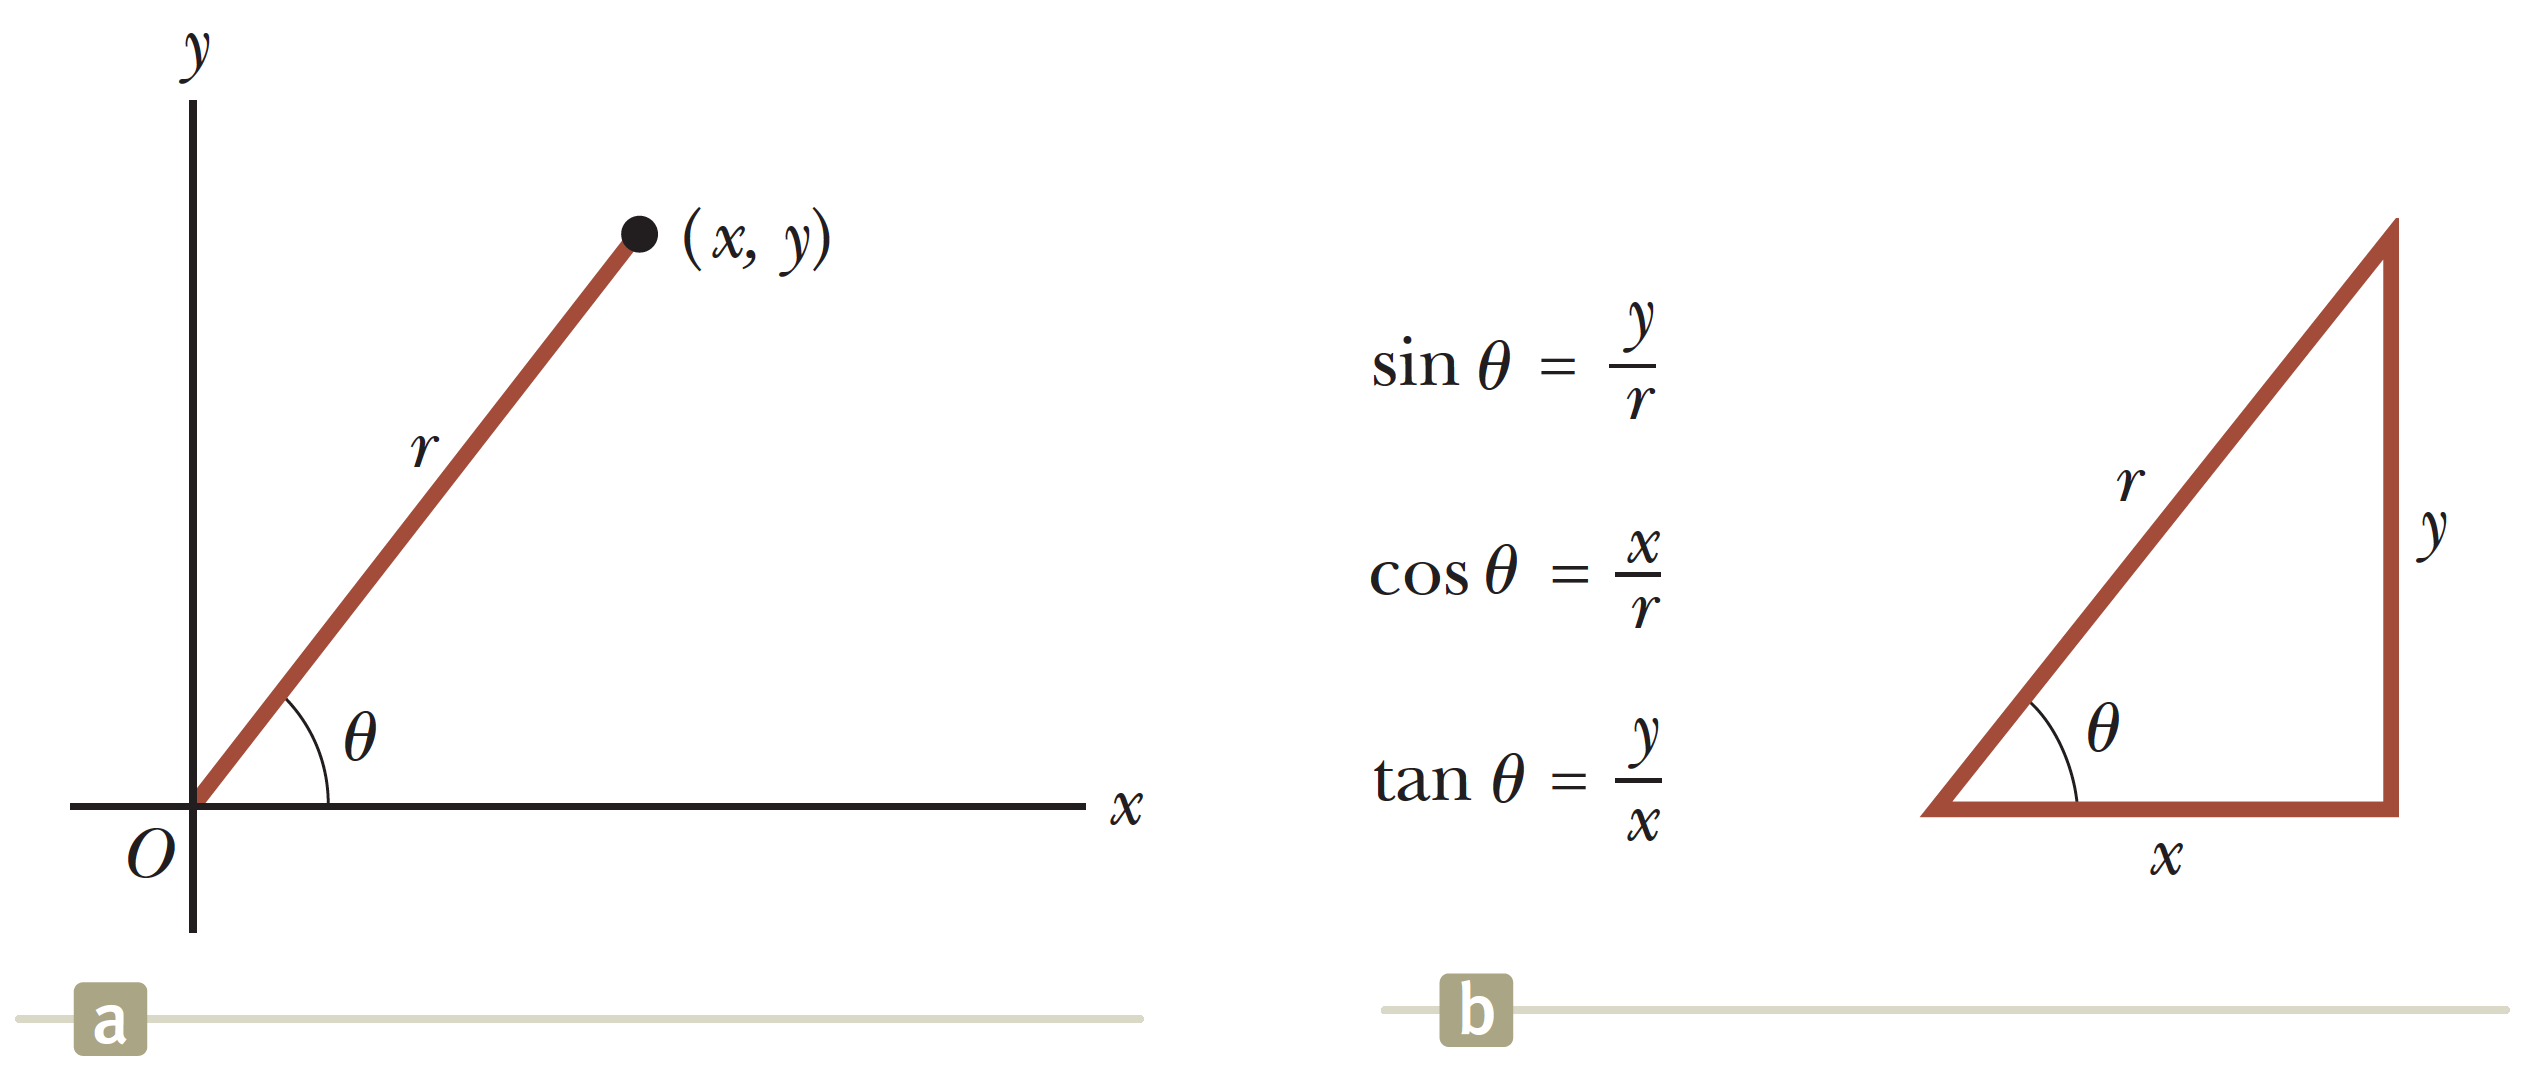
\includegraphics[scale=0.25]{1/graphics_3/figure_0}
      \caption{(a) Las coordenadas polares planas de un punto se representan mediante la distancia r y el ángulo u,
      donde u se mide contra el sentido de las manecillas del reloj a partir del eje x positivo. (b) El triángulo
      rectángulo se usa para relacionar (x, y) con (r, u).}
    \end{figure}

  \subsection{Cantidades vectoriales y escalares}
    \begin{itemize}
      \item Una \underline{cantidad escalar} se especifica por completo mediante un valor único con una unidad adecuada
        y no tiene dirección.
      \item Una \underline{cantidad vectorial} se especifica por completo mediante un número y unidades apropiadas más
        una dirección.
    \end{itemize}

  \subsection{Propiedades de los vectores}
    \begin{enumerate}
      \item \textbf{Igualdad de dos vectores:} $\BV{A} = \BV{B}$ sii $A = B$ y $\vec{A}, \vec{B}$ apuntan en la misma
        dirección.
      \item \textbf{Suma de vectores:} La suma de vectores es conmutativa y asociativa.
        \begin{figure}[H]
          \minipage{0.5\textwidth}
          \centering
          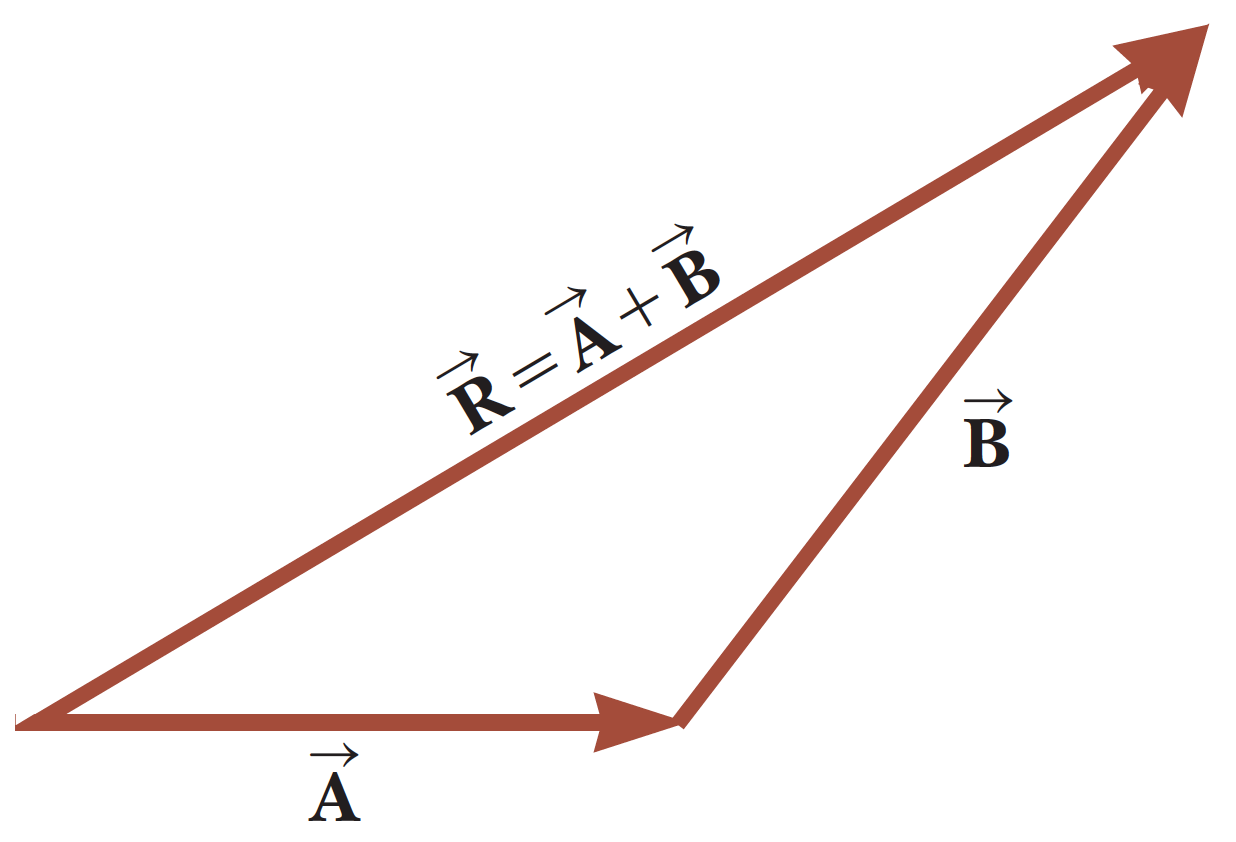
\includegraphics[scale=0.25]{1/graphics_3/figure_1a}
          \endminipage\hspace{0.8mm}
          \minipage{0.5\textwidth}
          \centering
          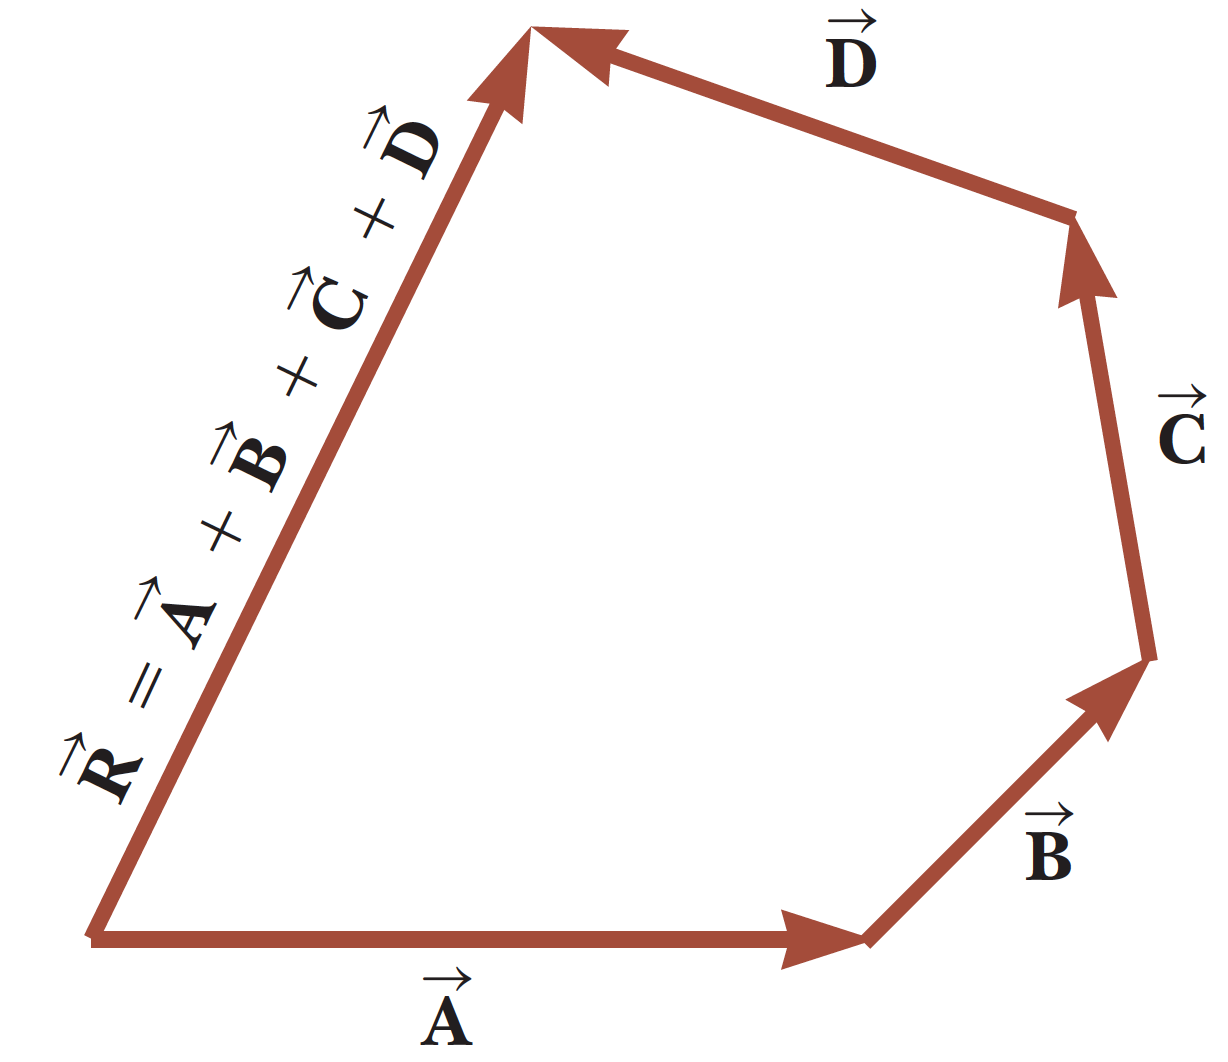
\includegraphics[scale=0.2]{1/graphics_3/figure_1b}
          \endminipage
        \end{figure}
      \item \textbf{Negativo de un vector:} El vector $-\BV{A}$ tiene la misma magnitud y dirección opuesta a $\BV{A}$.
      \item \textbf{Resta de vectores:}
        \begin{figure}[H]
          \centering
          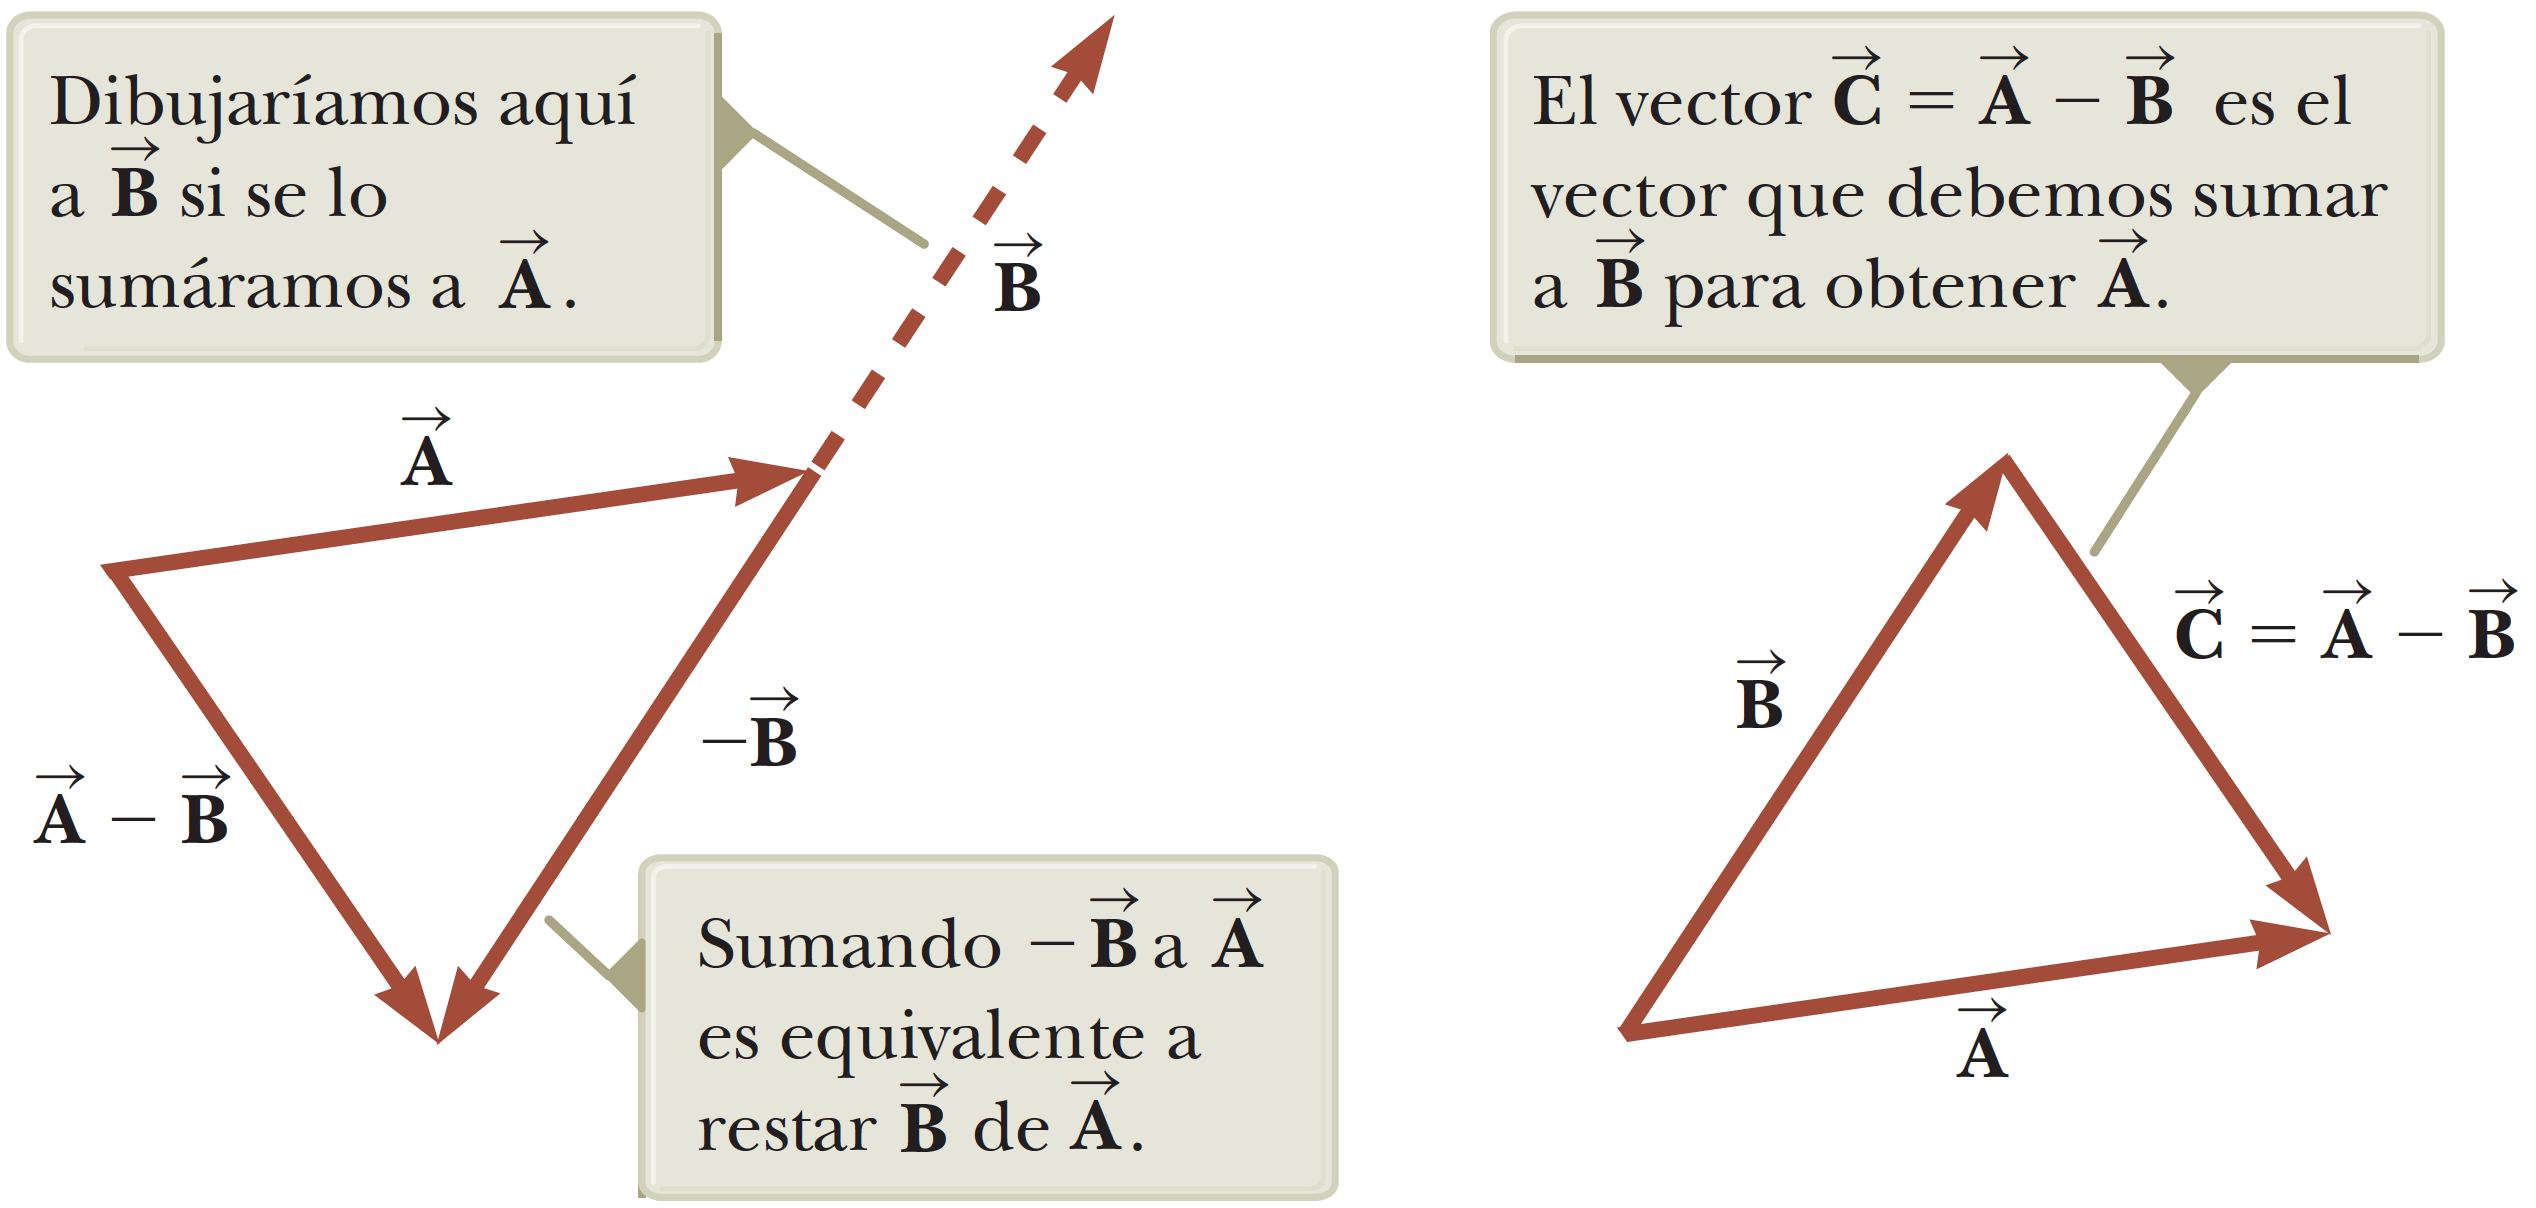
\includegraphics[scale=0.25]{1/graphics_3/figure_2}
        \end{figure}
      \item \textbf{Multiplicación de un vector por un escalar:} Si el vector $\BV{A}$ se multiplica por una cantidad
      escalar m, el producto $m\BV{A}$ es un vector que tiene la misma dirección que $\BV{A}$ y magnitud mA.
    \end{enumerate}

  \subsection{Componentes de un vector y vectores unitarios}
    \PN Un vector $\BV{A}$ se puede expresar como la suma de otros dos vectores componentes $\BV{A_{x}}$, que es
    paralelo al eje x, y $\BV{A_{y}}$, que es paralelo al eje y, ie, $\BV{A} = \BV{A_{x}} + \BV{A_{y}}$ y sus
    componentes, utilizando las definiciones de $\sin$ y $\cos$, son $A_{x} = A \cos \theta$ y $A_{y} = \sin \theta$.

    \begin{figure}[H]
      \centering
      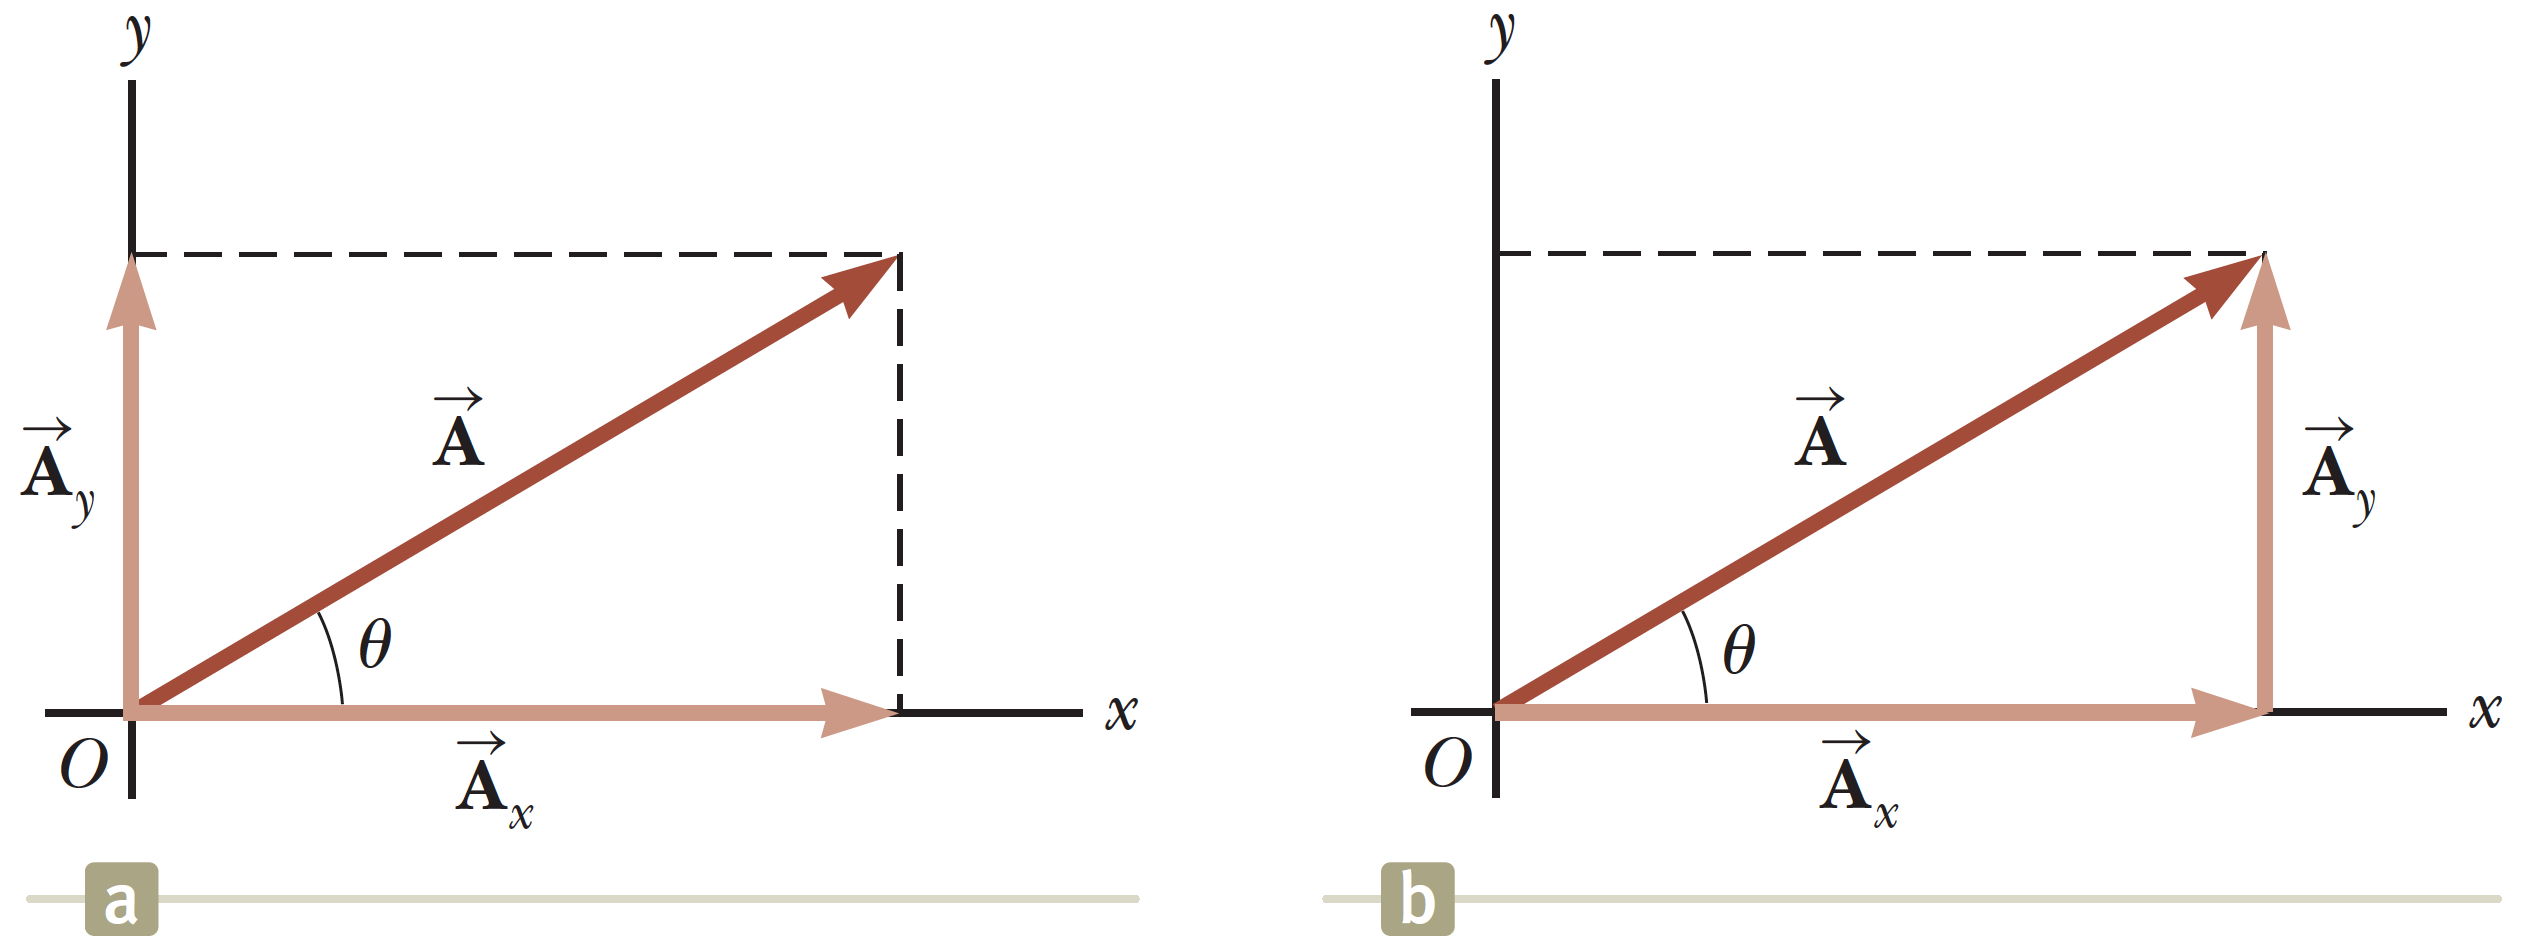
\includegraphics[scale=0.3]{1/graphics_3/figure_3}
    \end{figure}

    \subsubsection{Vectores unitarios}
      \PN Un \textbf{vector unitario} es un vector sin dimensiones que tiene una magnitud de exactamente 1. Los símbolos
      $\hat{i}, \hat{j}, \hat{k}$ se utilizan para representar los vectores unitarios que apuntan en las direcciones
      x, y, z respectivamente. La notación en vectores unitarios para $\BV{A}$ es:
      \[
        \BV{A} = A_{x} \hat{i} + A_{y} \hat{j}
      \]

      \PN La suma entre $\BV{A}$ y $\BV{B}$ en vectores unitarios es la siguiente:
      \[
        \BV{R} = (A_{x} + B_{x}) \hat{i} + (A_{y} + B_{y}) \hat{j}
      \]

      \begin{figure}[H]
        \centering
        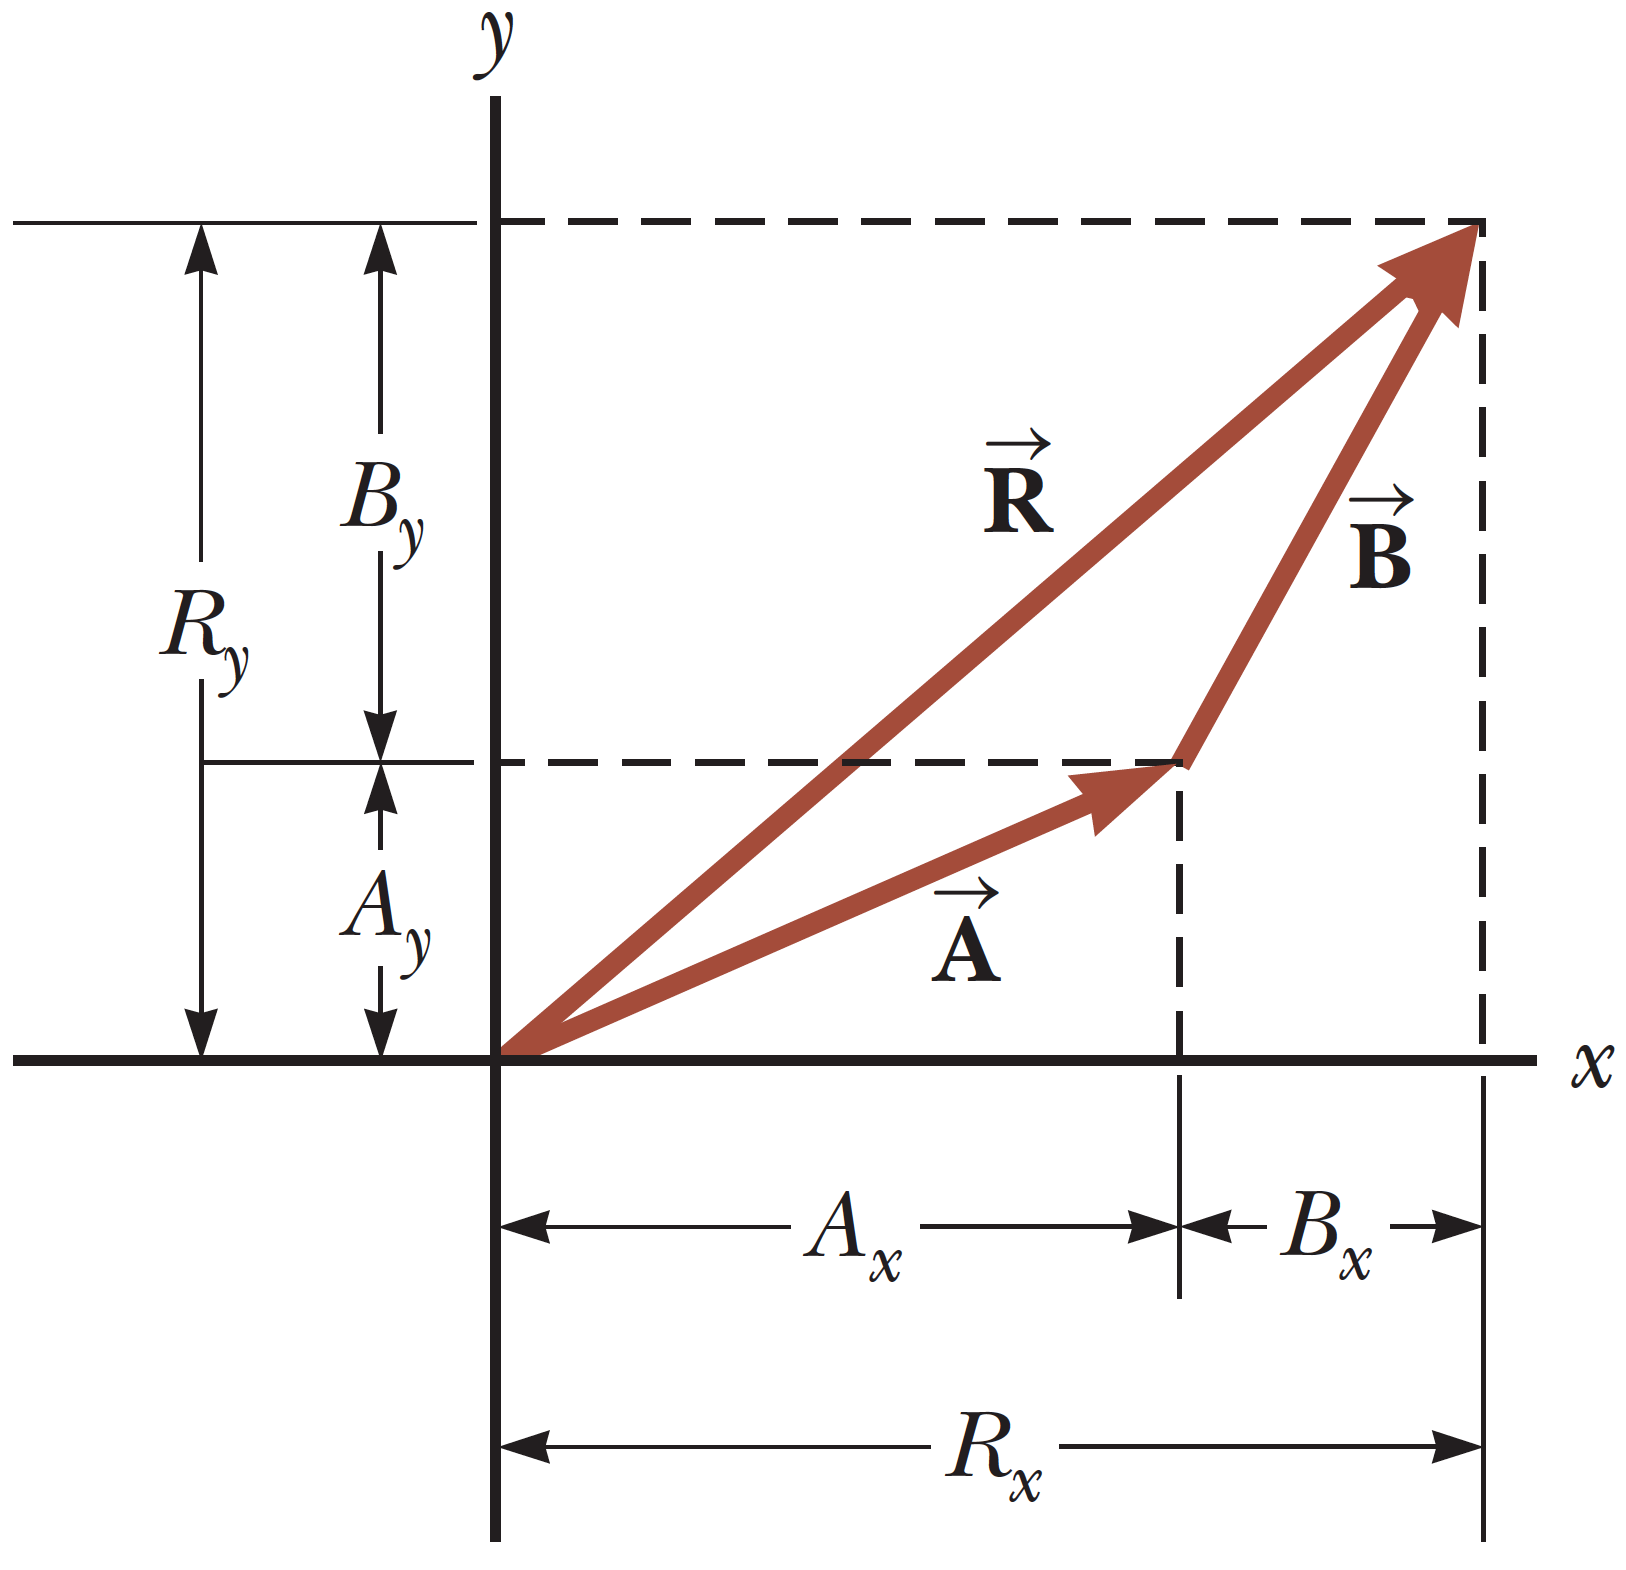
\includegraphics[scale=0.25]{1/graphics_3/figure_4}
        \caption{Esta construcción geométrica para la suma de dos vectores muestra la relación entre las componentes de
        la resultante $\BV{R}$ y las componentes de los vectores individuales.}
      \end{figure}
